Here is an alloy specification of the system described in the RASD: 
\vspace{2cm}
\lstinputlisting[language=alloy]{Alloy/RASD_ALLOY.als}
\newpage
% solo triangoli per le grandi


\begin{figure}[H]
    \begin{center}
        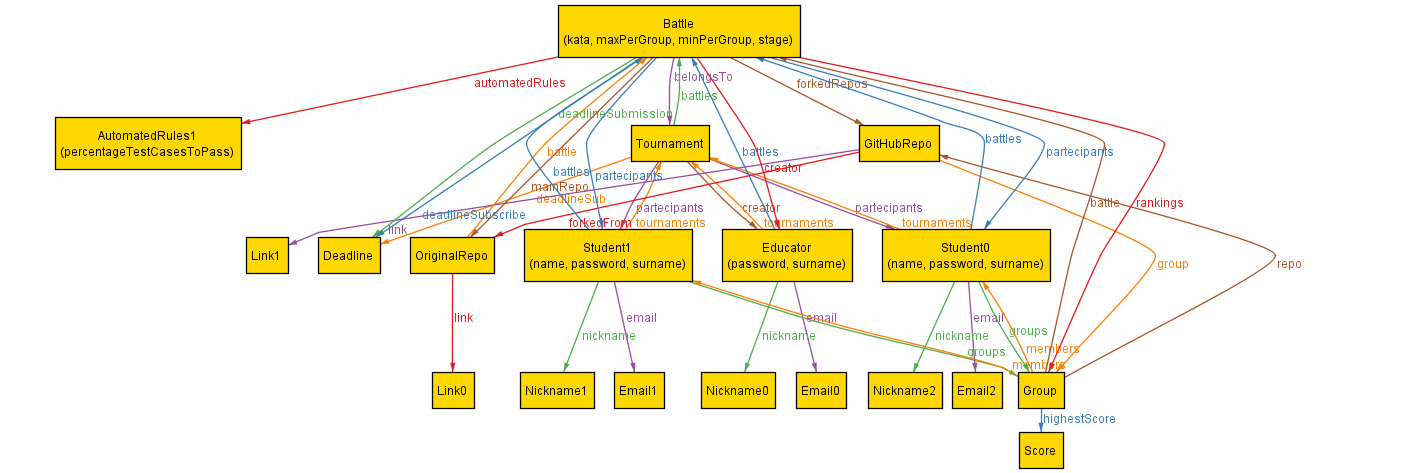
\includegraphics[width=1.2\linewidth]{AlloyIMG/baseWorld.png}
        \caption{Instance for \textit{baseWorld}.}
        \label{fig:baseWorld}%
    \end{center}
\end{figure}

\begin{figure}[H]
    \begin{center}
        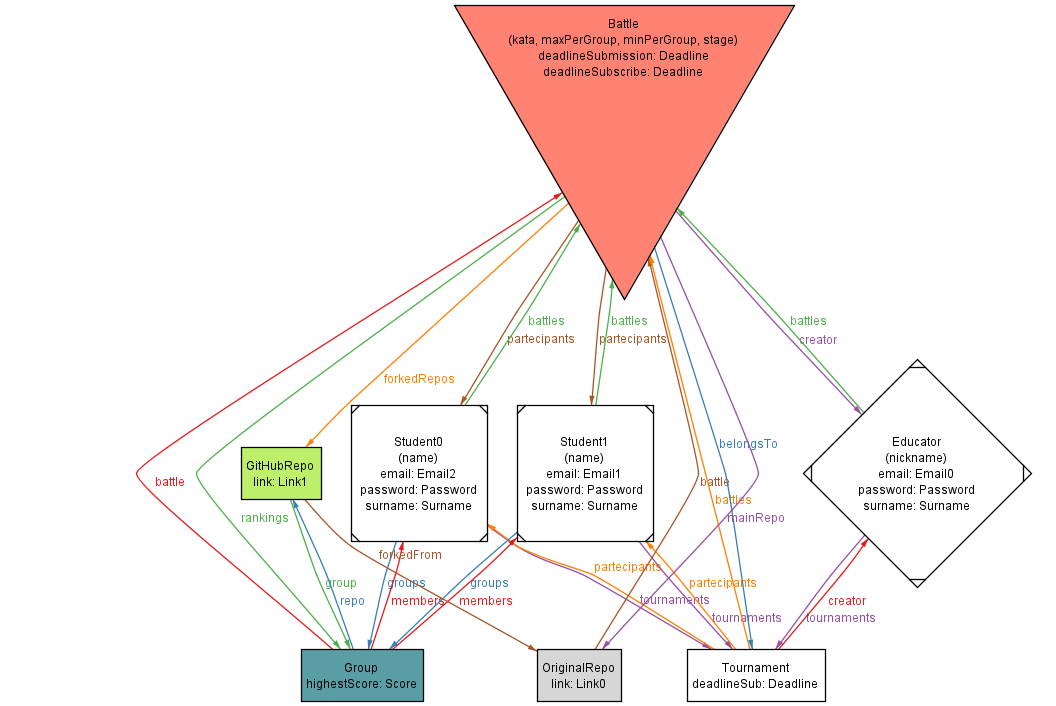
\includegraphics[width=1\linewidth]{AlloyIMG/baseWorld_magic.png}
        \caption{Simplified Instance for \textit{baseWorld}.}
        \label{fig:baseWorld_magic}%
    \end{center}
\end{figure}

\begin{figure}[H]
    \begin{center}
        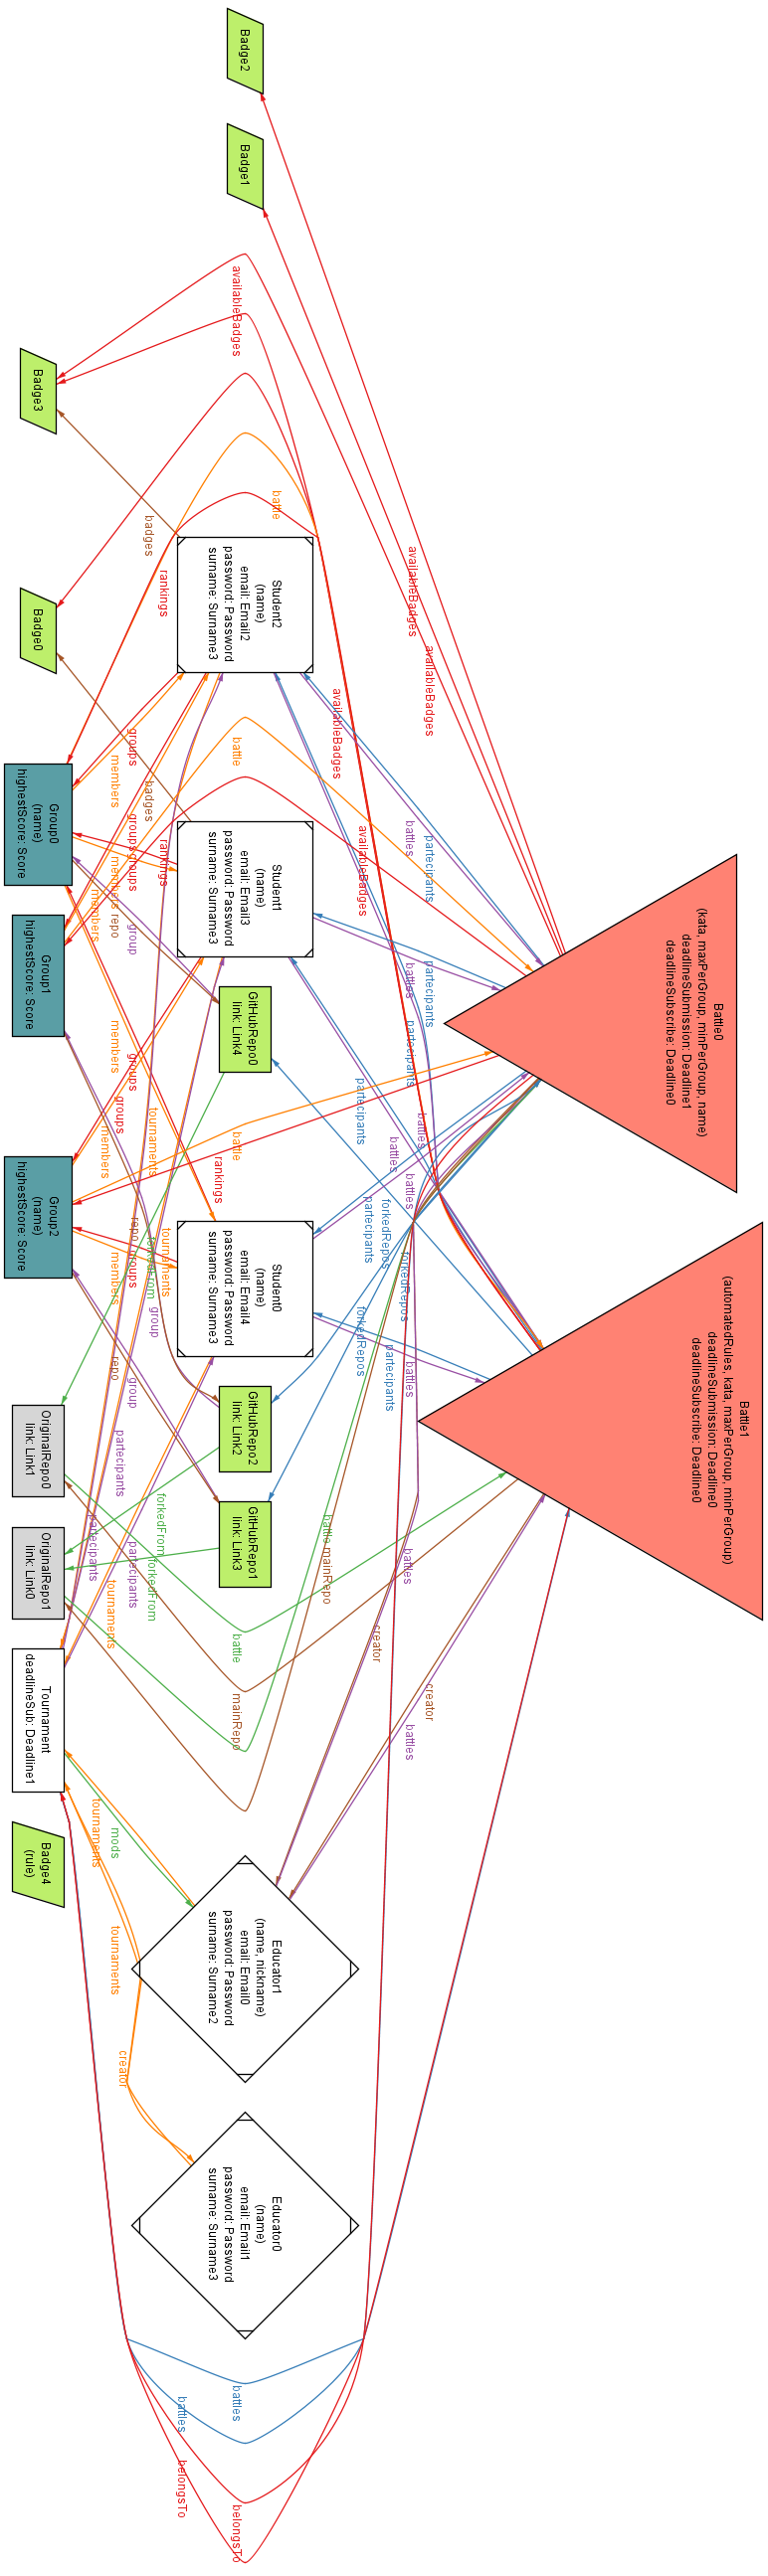
\includegraphics[width=0.4\linewidth]{AlloyIMG/world_magic.png}
        \caption{Simplified Instance for \textit{World}.}
        \label{fig:world_magic}%
    \end{center}
\end{figure}

\begin{figure}[H]
    \begin{center}
        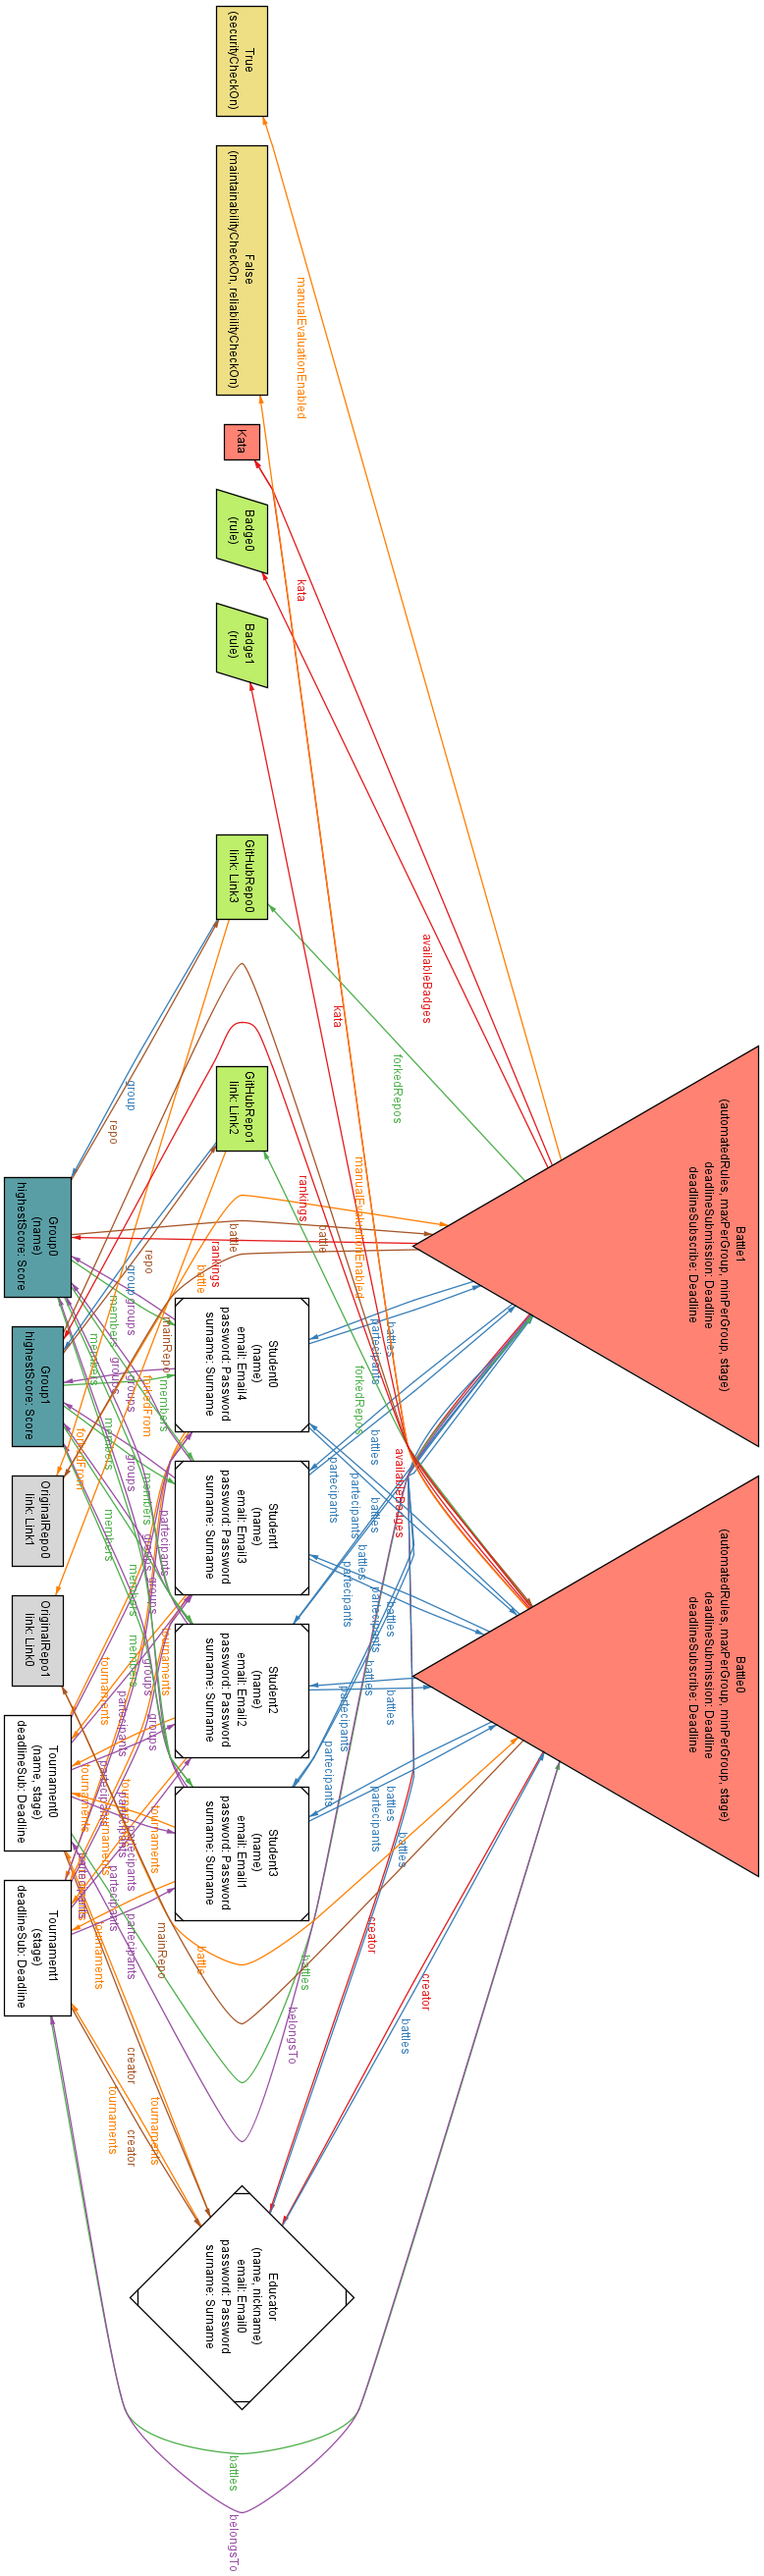
\includegraphics[width=0.4\linewidth]{AlloyIMG/world2_magic.png}
        \caption{Simplified Instance for \textit{World2}.}
        \label{fig:world2_magic}%
    \end{center}
\end{figure}
